\documentclass[../thesis/thesis.tex]{subfiles}
\renewcommand{\baselinestretch}{1.5}\selectfont
\graphicspath{{../figs/ch5-nlbmunc/}}

\begin{document}
	
\onlyinsubfile{\setcounter{chapter}{4}}

\begin{refsection}
\chapter[Prop. Meas. Unc. To Nonlinear Behavioural Models]{Propagating Measurement Uncertainty into Nonlinear Behavioural Models}
\section{Introduction}

A brief coverage of the requirement for behavioural models and the history. Talk about the benefits of adding confidence information to simulations during amplifier design.

yield analysis in circuit simulation
characterisation of amplifiers for digital pre-distortion \cite{Verspecht_2013,Kaur_2012}

Introduce black-box model definition with pseudowave equations.



\section{Nonlinear Behavioural Models}
\subsection{The Volterra ``VIOMAP'' Model}

One of the first examples of a nonlinear behavioural model for microwave amplifiers was the Volterra input-output map, or ``VIOMAP'' \cite{Verbeyst_1994}. This model was developed in the early nineties by Verbeyst and Vanden Bossche of the Hewlett Packard Network Measurement and Description Group (NMDG\footnote{now owned by National Instruments}) at Vrije University in Brussels. In an effort to find an S-parameter equivalent for nonlinear devices, VIOMAP replaces the parameters themselves with a sum of Volterra kernel components at each harmonic frequency\cite{Schetzen_2006, Moodi_2010}.

Although the VIOMAP model was shown to be cascadable \cite{Verbeyst_1994}, applicable across the Smith chart for efficient load-pull measurements \cite{Verbeyst_1995b}, and useful for characterising predistortion \cite{Verbeyst_1995}, it had two major shortcomings. Firstly, it could only be used to model weakly nonlinear devices. This issue was tackled by introducing orthogonal polynomials on which to base the Volterra kernel \cite{Verbeyst_1996}, although the choice of these polynomials was not clear to users and required a lot of computation, thus they were not widely adopted. Secondly, the measurement procedure was customised to suit different applications, which appeared to increase the barrier for entry to new users who could not confidently buy standard equipment to perform the measurements.

\subsection{Scattering Functions}

Scattering functions, originally termed describing functions from their nonlinear analysis origin, were introduced by Verspecht and reduced the computational overhead for modelling strong nonlinearities when compared to the VIOMAP model \cite{Verspecht_1996}. They are expressed as a function mapping $N$ complex numbers representing the input signal $I$ into the $k^{\textrm{th}}$ spectral component of the output signal $O$:

\begin{equation}
	O_{k} = F_k(I_1, I_2, \dots, I_N),
	\label{ch5_eqn_scatfunc}
\end{equation}

where $F_k$ is the scattering function for $k$. The VIOMAP model can be shown to be a subset of the scattering function approach, where the functions are constrained to a limited set of polynomials.

It should be mentioned here that all models described in this section require the device to be time-invariant, meaning that a time delay (or phase shift) in the input signal causes an equivalent time delay (or phase shift) in the output signal. This is typically the case for amplifiers, but more integrated communications components which include, for example, internal oscillators, cannot be modelled using the approaches described in this chapter.

Similar to the VIOMAP model, scattering functions are also complicated to apply and were not popular as a nonlinear modelling paradigm.

\subsection{Hot S-parameters}

Hot S-parameters were developed as a nonlinear behavioural model to extend S-parameters and allow stability and distortion characterisation of amplifiers \cite{Verspecht_2002, Verspecht_2005}. The model has several variations depending on the behaviour of interest, and there also exists an enhanced hot S-parameter model which incorporates additional information (in anticipation of the polyharmonic distortion model and the X-parameter model derived from it, which is described later).

Fundamentally, the hot S-parameter model, when used to characterise the distortion of amplifiers, provides a set of S-parameter measurements which are indexed against both frequency $f$ (like standard S-parameters) and also the amplitude of the incident tone $|a_1|$:

\begin{equation}
	\begin{bmatrix}
		b_1(f) \\ 
		b_2(f) 
	\end{bmatrix}
	= 
	\begin{bmatrix}
		hotS_{11}(f, |a_1|) & hotS_{12}(f, |a_1|) \\
		hotS_{21}(f, |a_1|) & hotS_{22}(f, |a_1|)
	\end{bmatrix}
	\begin{bmatrix}
	a_1(f) \\ 
	a_2(f) 
	\end{bmatrix}
\end{equation}

The enhanced version of the model includes two additional parameters which describe more completely the nonlinear output matching characteristic ($hotS_{22}$):

\begin{equation}
	\begin{bmatrix}
		b_1(f) \\ 
		b_2(f) 
	\end{bmatrix}
	= 
	\begin{bmatrix}
		hotS_{11}(f, |a_1|) & hotS_{12}(f, |a_1|) \\
		hotS_{21}(f, |a_1|) & hotS_{22}(f, |a_1|)
	\end{bmatrix}
	\begin{bmatrix}
		a_1(f) \\ 
		a_2(f) 
	\end{bmatrix}
	+
	\begin{bmatrix}
		T_{12}(f, |a_1|) \\ 
		T_{22}(f, |a_1|) 
	\end{bmatrix}
	e^{j\phi(a_1(f))}a_2^*(f)
	\label{ch5_eqn_hotsp}
\end{equation}

where $e^{j\phi(a_1(f))}$ normalises the phase of $a_2$ relative to $a_1$, $a_2^*$ is the conjugate of $a_2$ and $T_{ij}$ are the two new parameters in the enhanced model.

For an amplifier operating in the nonlinear regime, both the magnitude and phase of reflections at the output, due to matching, can have a significant impact on the device performance \cite[Figure 12.13]{Cripps_2006}. Figure \ref{ch5_fig_hots22} illustrates versions of the hot S-parameter model with different $hotS_{22}$ definitions.

The amplifier stability form of hot S-parameters will not be discussed here, but an overview is available in \cite{Verspecht_2005}.

\begin{figure}[t]
	\centering
	\includegraphics[width=\linewidth]{hots22}
	\caption[Performance of hot S-parameter models with different $hotS22$ definitions.]{Performance of hot S-parameter models with different $hotS22$ definitions, showing in polar form the measured (orange) and predicted (yellow) $b_2$ wave for a modulated large-signal $a_1$ wave, with values in Volts. Classic $S_{22}$ means no dependence of $S_{22}$ on $|a_1|$, simple ``Hot S22'' means a linear dependence of $S_{22}$ on $|a_1|$, extended ``Hot S22'' includes dependence of $S_{22}$ on $|a_1|$ and $a_2$, and quadratic ``Hot S22'' includes a second order dependence of $S_{22}$ on $a_2$ \cite{Verspecht_2002}.}
	\label{ch5_fig_hots22}
\end{figure}

\subsection{X-Parameters}

X-parameters, from Keysight, are the commercial realisation of the poly-harmonic distortion model \cite{Verspecht_2006}, which itself is an application of scattering functions with particular constraints. The most significant constraint is that any output of device which the model is applied to behaves linearly with respect to incident tones at harmonics of the fundamental, which is illustrated in Figure \ref{ch5_fig_superposition}. 

\begin{figure}
	\centering
	\includegraphics[width=0.65\textwidth]{superposition}
	\caption[The harmonic superposition principle.]{The harmonic superposition principle. If the input at port one ($A_1$) contains several small-signal harmonics, the output at port two ($B_2$) will comprise of the large-signal response plus the sum of responses due to each small-signal input harmonic, at each frequency \cite{Verspecht_2006}. The plots show complex phasors of increasing harmonic index along the horizontal axis, where the colour of the output phasors relate to the contribution from the respective input phasor.}
	\label{ch5_fig_superposition}
\end{figure}

The X-parameter formulation can be developed from the scattering function origin. Firstly, the output $B_{p, k}$, at port $p$ and harmonic $k$, is defined as:

\begin{equation}
	B_{p, k} = \sum_{q,l}S_{p, k;q, l}(|A_{1,1}|)P^{k-l}A_{q, l} + 
	\sum_{q,l}T_{p, k;q, l}(|A_{1,1}|)P^{k+l}A_{q, l}^*,
\end{equation}

where $A_{q,l}$ is the input at port $q$ and harmonic index $l$, and $P$ is a phase normalisation coefficient such that $P=e^{j\phi(A_{1,1})}$, similar to (\ref{ch5_eqn_hotsp}). This equation contains two scattering functions which are sensitive to the large-signal input at the fundamental, $A_1,1$. The second function, $T_{p, k;q, l}$, is identical to $S_{p, k;q, l}$ except that it is a coefficient of the conjugate of the input wave, $A_{q, l}^*$. As with the enhanced Hot S-parameters, this is a more generalised way to incorporate the sensitivity of the model to the phase of input signals at harmonics on any port. Mathematically, the requirement of these two functions is a result of the non-analyticity of the complex-valued scattering functions. It is possible to instead define the functions in terms of real and imaginary components, but the normal and conjugate definition is standard for X-parameters and so will be taken forward here.

Because the phase is normalised with respect to that of $A_{1, 1}$, we can also define $T_{p,k;1,1}=0$ as the entire device response for this port and harmonic combination will be captured in $S_{p,k;1,1}$, which also represents the response to the large-signal input at port one at the fundamental tone. If we assume that the harmonic superposition principle is valid for our model, we can then simplify it by extracting the large-signal response as a separate term and treat the remaining functions as linear, with the restriction that they do not apply when $q, l = 1, 1$. A good overview of this linearisation process of scattering functions is provided in \cite{Verspecht_2005b}.

We can now write our model as:

\begin{equation}
\begin{split}
B_{p, k}=X^\textrm{F}_{p, k}(|A_{1, 1}|)P^k+\sum_{q, l\ne(1,1)}[X^\textrm{S}_{p, k;q, l}(|A_{1, 1}|)A_{q, l}P^{k-l}\\+X^\textrm{T}_{p, k;q, l}(|A_{1, 1}|)A^*_{q, l}P^{k+l}],
\end{split}
\label{ch5_eqn_xps}
\end{equation}
where $X^\textrm{F}$ (the large-signal term), $X^\textrm{S}$ and $X^\textrm{T}$ (the small-signal terms) are called X-parameters.

Two informative comparisons between the performance of scattering functions and X-parameters in modelling nonlinear device behaviour can be found in \cite{Sun_2010,Widemann_2015}.

The X-parameter model is heavily marketed by Keysight to be a complete solution for modelling nonlinear device behaviour. Additions to the model include the ability to measure performance at a full range of load impedances (by making the X-parameters a function of $A_{2,1}$ also) \cite{Gunyan_2009}, mixer characterisation using multi-tone stimuli \cite{Xie_2012}, the inclusion of memory effects \cite{Verspecht_2009}, the prediction of load-pull performance from a single X-parameter measurement at 50-Ohms \cite{Root_2017}, and recently the inclusion of electro-thermal effects \cite{Gillespie_2018}.

\subsection{The Cardiff Model}

Although X-parameters are sufficient to characterise the nonlinear behaviour of many amplifiers, the standard model\footnote{It is possible to extend the X-parameter model to include higher order mixing products, however this is not supported by commercial measurement or simulation solutions.} only includes third-order mixing products (via the $P^{(.)}$ terms in (\ref{ch5_eqn_xps})). For strongly nonlinear devices, such as unpackaged transistors and amplifiers driven in class F modes, this limitation can be a cause for concern and lead to significant inaccuracies during simulations. The Cardiff model, named after it's origin at Cardiff University, UK, removes this limitation and incorporates $n^{\textrm{th}}$-order mixing products (typically truncated to seventh-order terms) \cite{Woodington_2008,Qi_2009}.

The formulation of the Cardiff model is represented differently to that of X-parameters, however, they are a natural extension of that model and are equivalent when used with third-order mixing products. The measurement and extraction process is usually performed with a sampler-based NVNA featuring a real-time sampling oscilloscope and consists of a load-pull measurement \cite{Woodington_2010}.

For this project, X-parameters were chosen as the nonlinear behavioural model for which to focus on developing an uncertainty propagation, due to their current popularity. The framework which has been developed can be extended to include other models, but does not currently support them. Therefore, the Cardiff model will not be discussed in any greater detail here.

\section{X-Parameter Extraction Procedure}
\subsection{Model}
\subsection{Uncertainty Propagation Using The MUF}
\section{Design and Simulation using Nonlinear Behavioural Models Incorporating Measurement Uncertainty}

The NIST MUF was used to perform the calibration of electromagnetic wave parameters measured using a Keysight Technologies 67 GHz N5247A PNA-X LSNA. The DUT was an internally matched Analog Devices HMC342LC4 low noise amplifier \cite{hittite_amp} mounted on a connectorised evaluation board. This amplifier has a typical gain of 19 dB and a \mbox{1-dB} compression point at approximately 9 dBm output power at 25 GHz. To obtain results showing both the linear and nonlinear regimes of operation, the source power was swept between -22 dBm and -2 dBm in 0.25 dB steps. The fundamental frequency was set at 25 GHz, with a harmonic at 50 GHz also measured. The evaluation board used 2.92 mm precision connectors, connected via adapters to cables with 2.4 mm precision connectors. The calibration plane was located between the cables and the adapters (i.e. the adapters were included as part of the DUT), and the measurement setup had a nominal impedance of 50-$\Omega$. The intermediate frequency bandwidth (IFBW) was set to 10 Hz. The built-in X-parameter measurement routine was used and configured to extract cross-frequency terms between both harmonics using measurements at 4 extraction tone phases (this is the default setting). A photograph of the setup is shown in \figurename{ \ref{ch5_fig_setup}}.

\begin{figure}[t]
	\centering
	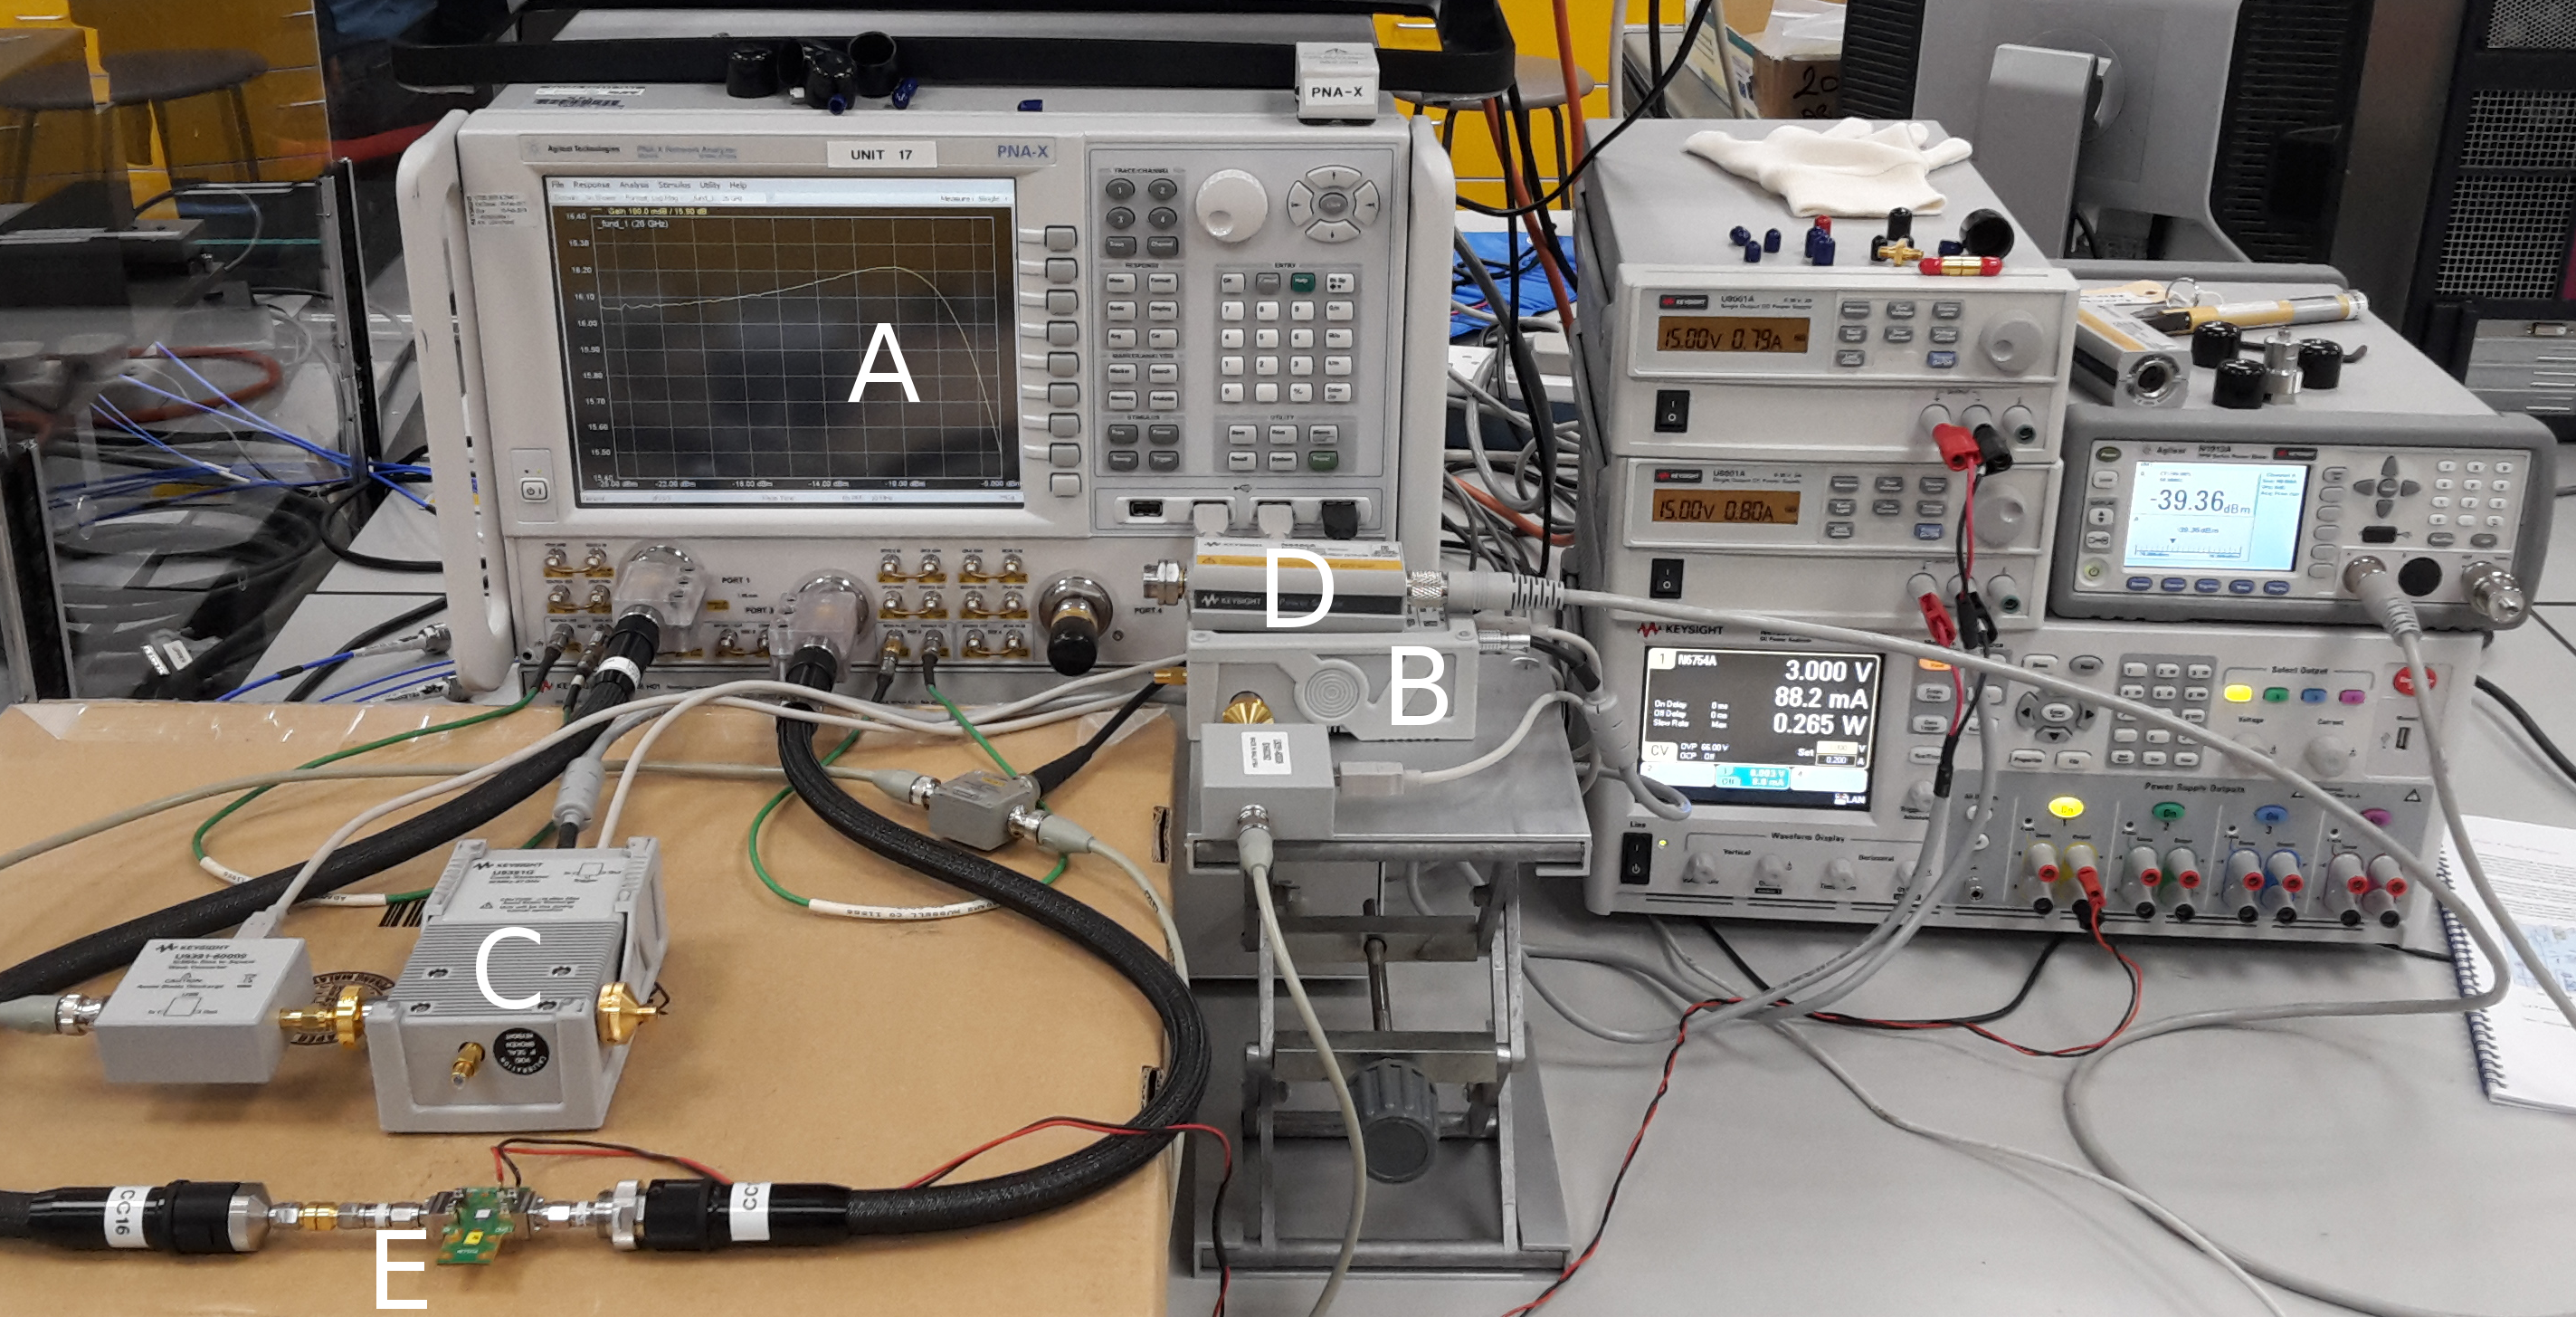
\includegraphics[width=\linewidth]{setup}
	\caption{The measurement setup used for extracting X-parameters from the DUT. Shown is the PNA-X LSNA (A), the phase reference comb generator (B), the phase calibration comb generator (C), the power meter (D), and the connected DUT (E).}
	\label{ch5_fig_setup}
\end{figure}

Uncertainties are propagated through all steps of the calibration by the MUF. We have included uncertainties present in the definitions and measurements of the passive calibration standards, the power meter calibration and measurement, the phase reference characterization and measurement, cable flexure, and connection repeatability of all calibration steps. Uncertainty due to random noise in the high-dynamic range receivers was omitted as it has been shown to be negligible with respect to that arising from other error sources in LSNA measurements \cite{Blockley_2007}.

The MUF supports several calibration algorithms, and for this measurement the multiline TRL calibration algorithm \cite{Engen_1979, Marks_1991} was chosen to allow direct dimensional traceability to national measurement standards. The calibration standards used were from a 1.85 mm precision coaxial calibration kit (Rosenberger RPC-1.85 LRL). Table \ref{ch5_table_passivestds} gives the dimensions of the line standards used for the calibration. To include the effect of connector repeatability on the passive calibration, each standard was measured several times with the connector oriented differently. These measurements were passed to a MUF program (``Combine'') which produces a mean value with an associated uncertainty.

\begin{table}[]
	\centering
	\caption{Nominal values and standard uncertainties for the TRL coaxial line standards.}
	\label{ch5_table_passivestds}
	\begin{tabular}{ccc}
		\hline
		Dimension         & Line 1 value (mm) & Line 2 value (mm) \\ \hline
		Line length       & 13.004 $\pm$ 0.003 & 14.913 $\pm$ 0.003 \\
		Line inside dia.  & 0.803 $\pm$ 0.001 & 0.803 $\pm$ 0.008 \\
		Line outside dia. & 1.850 $\pm$ 0.005 & 1.850 $\pm$ 0.005 \\ \hline            
	\end{tabular}
\end{table}

The power meter measurement, as part of the absolute calibration, measures the amplitude of the waves. The calibration model for the power meter itself is defined in \cite{Keysight_2017} and includes the reference oscillator mismatch, the reference oscillator power uncertainty, the zero-set error, the zero carry-over error, the instrumentation error, and error in the power sensor calibration factor. The estimates and uncertainties used for these parameters in the calibration are shown in Table \ref{ch5_table_powerunc} and are derived from specifications supplied by the manufacturer. The mismatch of the power sensor was also measured using a calibrated VNA and included in the absolute calibration. Connector repeatability was assessed for this measurement in the same way as for the passive standards.

\begin{table}[]
	\centering
	\caption{Standard uncertainties for power meter uncertainty contributions derived in \cite{Keysight_2017}}
	\label{ch5_table_powerunc}
	\begin{tabular}{cc}
		\hline
		Contribution                           & Standard uncertainty \\ \hline
		Reference oscillator mismatch          & 0.2\%                \\
		Reference oscillator power uncertainty & 0.6\%                \\
		Zero-set error                         & 0.5\% meter full scale \\
		Zero carry-over error                  & 0.2\% meter full scale \\
		Instrumentation error                  & 0.5\% meter full scale \\
		Calibration factor error               & 0.024               \\ \hline
	\end{tabular}
\end{table}

In order to complete the absolute calibration, the phase must also be calibrated. This is performed using a harmonic phase reference, which for this calibration was provided by a Keysight Technologies 67 GHz comb generator\cite{Keysight_2014}. This device supplies a stable and repeatable train of pulses, which creates a frequency comb (aligned to the calibration frequencies) to be measured by the LSNA. The phase uncertainties are given in Table \ref{ch5_table_phaseunc} and were obtained through characterization with a sampling oscilloscope at NIST, which is traceable to national measurement standards via electro-optic calibration \cite{Reader_2008, Hale_2009}.

\begin{table}[]
	\centering
	\caption{Nominal phase and standard uncertainty for harmonic phase reference at calibration frequencies}
	\label{ch5_table_phaseunc}
	\begin{tabular}{ccc}
		\hline
		Frequency (GHz) & Characterized phase (deg.) & Measured phase (deg.)\\ \hline
		25 & 181.5 $\pm$ 0.4 & -16.8 $\pm$ 1.5 \\ 
		50 & 170.8 $\pm$ 1.0 & 61.0 $\pm$ 2.5 \\ 
		\hline
	\end{tabular}
\end{table}

\subsection{X-Parameter Uncertainties}

In this example we used Monte Carlo with 1000 samples to propagate uncertainty to the X-parameters of the DUT. This required 8 hours of processing for the calibration and a further 8 hours of processing for the X-parameter extraction.
A histogram is provided in \figurename{ \ref{ch5_fig_hist}} showing good agreement between the Monte Carlo and sensitivity analysis. This level of agreement is typical for all of the extracted X-parameters.

The estimated values and standard uncertainties from the Monte Carlo analysis for the magnitude and phase of a sample of X-parameter terms are shown in \figurename{ \ref{ch5_fig_summaryplots}}. It can be seen in all plots that there is a clear change in uncertainty for several X-parameters as the DUT transitions between the linear and nonlinear regimes.

The phase noise seen at lower powers in the estimate of $X^\textrm{T}_{2,1;2,2}$ is not accompanied by an increase in measurement uncertainty. This suggests that it arises from the extraction routine, which contributes another source of uncertainty not studied in this paper. By design, the $X^\textrm{T}$ parameters are negligible in the linear regime, and so this effect will have little contribution when the model is used.

\begin{figure}
	\centering
	\includegraphics[width=0.8\textwidth]{hist}
	\caption{Histogram comparing the Monte Carlo and sequential perturbation uncertainty results for $X^\textrm{S}_{2,1;2,1}$ (25 GHz) of the DUT at -2.4 dBm source power. The vertical line in the center of the plot (A) shows the nominal value (estimate), (B) shows the Monte Carlo average, and (C, D) show the Monte Carlo and sequential perturbation 95\% confidence intervals, respectively.}
	\label{ch5_fig_hist}
\end{figure}

\begin{figure}
	\centering
	\begin{subfigure}{0.45\textwidth}
		\includegraphics[width=\linewidth,height=5cm]{fig4a}			
		\label{ch5_fig_FB1kdB}
	\end{subfigure}\hfil%
	\begin{subfigure}{0.45\textwidth}
		\includegraphics[width=\linewidth,height=5cm]{fig4b}
		\label{ch5_fig_FB1kp}
	\end{subfigure}
	\begin{subfigure}{0.45\textwidth}
		\includegraphics[width=\linewidth,height=5cm]{fig4c}
		\label{ch5_fig_s212kdB}
	\end{subfigure}\hfil%
	\begin{subfigure}{0.45\textwidth}
		\includegraphics[width=\linewidth,height=5cm]{fig4d}	
		\label{ch5_fig_t212kp}
	\end{subfigure}
	\caption{Estimates (solid line and shapes, left scale) and standard uncertainties (dashed line and hollow shapes, right scale) for the magnitude and phase of a sample of the extracted X-parameters. Harmonic indices 1 and 2 relate to measurement frequencies of 25 and 50 GHz, respectively. Uncertainties are a linear variation of the scale value.}
	\label{ch5_fig_summaryplots}
\end{figure}

\section{Conclusions}

\addcontentsline{toc}{section}{Bibliography}
\printbibliography[title=References]
\end{refsection}
\end{document}
